\documentclass[final]{svjour2}
\usepackage{amsmath}
\usepackage{graphicx}
\usepackage{rotating}
\usepackage{amssymb}
\usepackage{mathptmx}
\usepackage[numbers]{natbib}
\usepackage{float}
\usepackage[section]{placeins}
\usepackage{tabularx}
\usepackage{booktabs}
\usepackage{color}
\makeatletter
\journalname{Journal of Low Temperature Physics}
%%%%%%%%%%%%%%%%%%%%%%%%%%%%%% Textclass specific LaTeX commands.
%%%%%%%%%%%%%%%%%%%%%%%%%%%%%% User specified LaTeX commands.
\bibpunct{}{}{,}{s}{}{,}

\begin{document}

\newcommand{\hdblarrow}{H\makebox[0.9ex][l]{$\downdownarrows$}-}
\title{Material Selection for Cryogenic Support Structures}

\author{E. Kramer \and N. Kellaris  \and M. Daal \and N. Zobrist \and S. Govindjee \and B. Sadoulet \and S. Golwala \and M. Hollister}

\institute{Department of Physics, U.C. Berkeley,\\ Berkeley, CA 94709, USA\\
\email{ekramer@berkeley.edu}}

\date{07.29.2013}

\maketitle

\begin{abstract}

Design specifications for the support structures of low temperature instrumentation often call for low thermal conductivity between temperature stages, high stiffness, and specific load bearing capabilities. Common design solutions employ thin-walled tubes and truss structures.  While overall geometric design plays an important role in both overall strength and heat flux between stages, material selection can affect a structure's properties significantly.  In this contribution, we suggest and compare several alternative materials to the current standard materials for building cryogenic support structures.

\keywords{Cryogenic Tower, Thermal Conductivity, Material Strength}
 
\end{abstract}

\section{Introduction}
Both slender member truss and thin-walled tube structures exhibit desirable qualities for low temperature instrumentation support structures due to their designs allowing for high structural stiffness and low heat flux across temperature stages.  Designing optimal structures that obtain the lowest thermal conductivity between temperature stages while still remaining structurally adequate to support  forces while in use at base temperature and while handling at room temperature is a optimization problem.  While the actual physical design geometry plays a major role in the overall effectiveness of a structure, material selection is just as important.  Unlike design geometry alterations, a change of material used to build a structure tends to be a much easier and predictable way to improve upon a design in terms of its performance under a force or heat load. Another advantage of material selection in terms of optimization comes in the form of theoretical equations and computer simulation for a structure's projected performance.  Unlike geometric changes to a structures shape, a change in the material used does not necessitate a change in the governing equations or model for theoretical evaluation due to the fact that material properties tend to be well defined dependent variables in both.  Material selection is also an important factor to keep in mind when it comes to a structure's non-ideal performance in the lab. Under non-ideal circumstances, materials and structures typically fail before their theoretical yield or break point due to imperfections, including but not limited to impurities or microscopic fractures introduced while processing the material.

\section{Material Selection Design Parameters}

Materials are defined by specific properties which are theoretically identical for all specimens of a single material type.  In actuality, these material properties deviate slightly from sample to sample due to differences in manufacturing, however the deviation is negligible for high quality production.  There are a few main properties that are of interest when creating cryogenic tower support structures.  The main structural property is the material's Youngs Modulus.  Youngs Modulus is a property that directly defines a materials stiffness or elasticity.  Materials with high Youngs Modulus are better suited for creating stiff structures because they deform less under load than materials with lower ones.  Youngs Modulus can be further broken down into compressive and tensile modulus for non isometric materials. Other structural properties of interest include both tensile and compressive strength which define the materials ability to withstand an applied force, in tension and compression respectively, without failing through plastic deformation or fracture.  While not defined by a specific property, the type of material (brittle or ductile) should also be taken into account due to the fact that buckling tends to occur before the onset of other failure modes in slender samples of non-brittle materials.  

Materials cannot be solely selected on their structural properties however, as thermal resistivity between stages is also a concern in cryogenic support structures. Thermal conductivity is a concern, which narrows down a large number of stiff materials that typically are used in non-cryogenic application structures.  Overall materials must be stiff enough to not fail under expected loads ranges while keeping their cross section as low as possible to minimize the amount of heat transfer between temperature stages.  In general when choosing materials we desire the smallest Thermal conductivity to Youngs Modulus ratio.\cite{Hastings1993}  

\section{Property Results of Useful Materials}

A variety of materials exist with acceptable strength and thermal properties for use in a cryogenic support structure setting.  In the plot and table below we present a few newer useful materials along with industry standard ones that have a low thermal conductivity to Youngs Modulus ratio.\cite{Doty1981}\cite{Kasen1981}\cite{Runyan2008}\cite{Kellaris2013}\cite{Woodcraft2009}\cite{Woodcraft2009_2}\cite{Ventura2009}

\begin{figure}[!ht]
\begin{center}
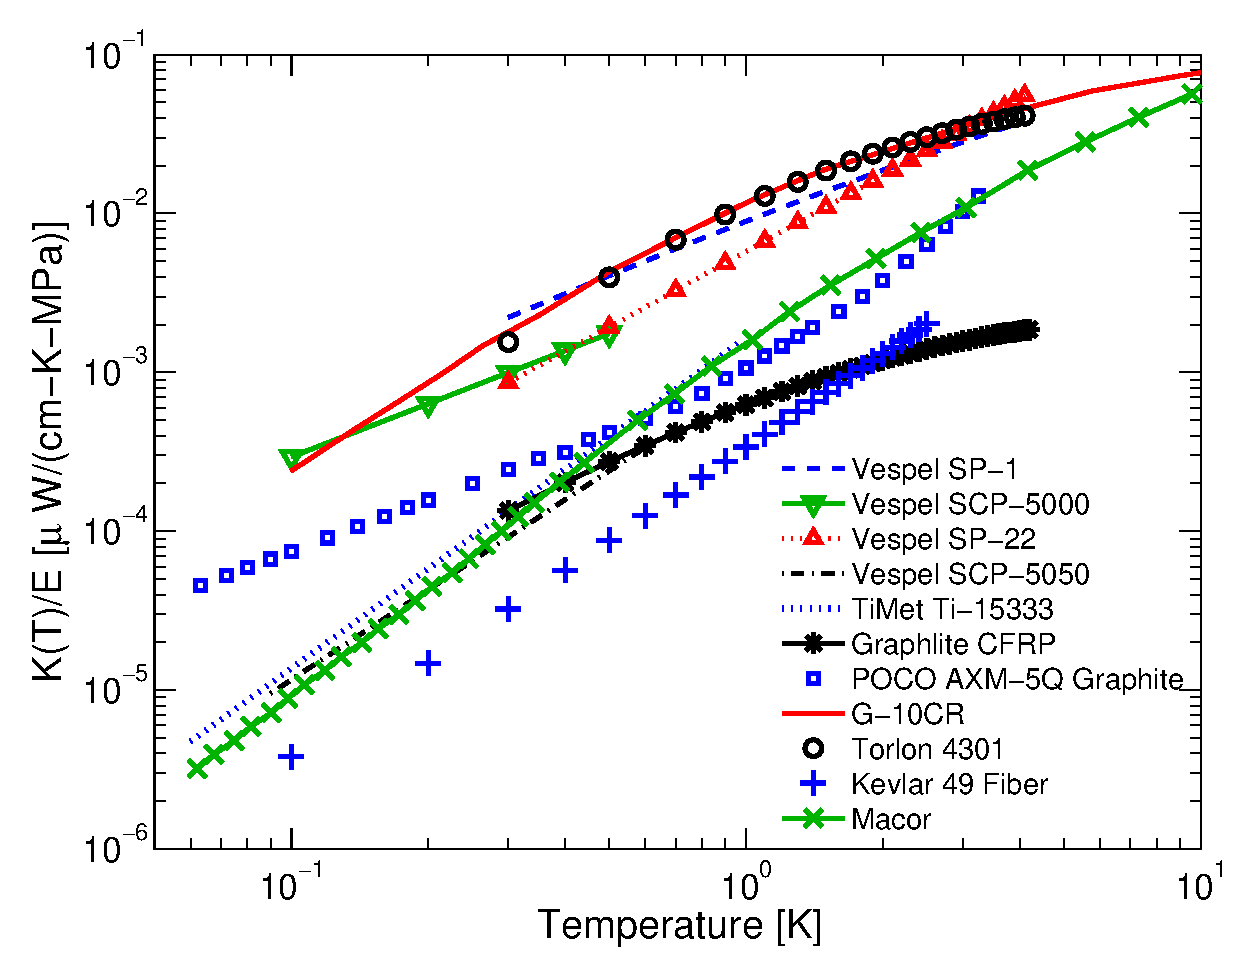
\includegraphics[%
  width=0.95\linewidth,
  keepaspectratio]{Mats}
\end{center}
\caption{A selection of popular and useful materials with their room temperature Youngs modulus normalized by their thermal conductivity.  Lower values correspond to materials with lower thermal conductivity to stiffness ratio, thus making them more ideal materials for support structures.}
\label{Mats}
\end{figure}

\begin{figure}[!ht]
\begin{center}
\includegraphics[%
  width=0.85\linewidth,
  keepaspectratio]{Table}
\end{center}
\caption{Material strength properties of some select materials at room temperature.}
\label{SW}
\end{figure}

\section{Conclusions}
While many different geometric design solutions are available when creating cryogenic support structures, material selection plays a vital role in allowing structures to remain strong while providing low heat loads between stages.  It is important to pick the material to cater specifically to the design specifications of the structure as some materials are better suited than others under specific load types.  The value of interest is the thermal conductivity of a material normalized to its strength, which for simplicity is typically the Youngs modulus, however other parameters for material strength can be used if the design calls for them.

\begin{acknowledgements}
We would like to thank S. Govindjee for technical assistance. We acknowledge support and funding from the Department of Energy and the National Science Foundation.
\end{acknowledgements}

\begin{thebibliography}{99}

%%%%%%%%% Structure bibliography items %%%%%%%%%%
%%%%%%%%%%%%%%%%%%%%%%%%%%%%%%%%%%%%%%%%%%%%%%%%%
\bibitem{Hastings1993}
Peter R. Hastings and D.M. Montgomery. Support of cooled components in astronomical instruments. Cryogenics, 33(11):1032–1036, 1993.

%%%%%% Young's modulus bibliography items %%%%%%%%%
%%%%%%%%%%%%%%%%%%%%%%%%%%%%%%%%%%%%%%%%%%%%%%%%%%%

\bibitem{Doty1981}
F.D. Doty and P.D. Ellis, {\it Rev. Sci. Instrum.} \textbf{52(12)}, 1868, (1981).

\bibitem{Kasen1981}
M.B. Kasen, G.R. MacDonald, D.H. Beekman, Jr., and R.E. Schramm, {\it Advances in Cryogenic Engineering Materials} \textbf{26}, 235, (1981). 

%%%% Thermal conductivity bibliography items %%%%
%%%%%%%%%%%%%%%%%%%%%%%%%%%%%%%%%%%%%%%%%%%%%%%%%

%%% Vespel SP-1, Vespel SP-22, Graphlite CFRP, Torlon 4301
\bibitem{Runyan2008}
M.C. Runyan and W.C. Jones, {\it Cryogenics} \textbf{48}, 448, (2008).

%%% Vespel SCP-5000, Vespel SCP-5050, Ti 15-3-3-3
\bibitem{Kellaris2013}
N.A. Kellaris. {\it Unpublished thermal conductivity measurements}, (2013).

%%% AXM-5Q
\bibitem{Woodcraft2009}
A.L. Woodcraft, M. Barucci, P.R. Hastings, L. Lolli, V. Martelli, L. Risegari, and G. Ventura, {\it Cryogenics} \textbf{49}, 159, (2009).

%%% G-10CR & Macor
\bibitem{Woodcraft2009_2}
A.L. Woodcraft and A. Gray, {\it Low Temp. Detectors 13, Proceedings of the 13$^{th}$ International Workshop}, \textbf{1185}, 681, (2009).

%%% Kevlar 49
\bibitem{Ventura2009}
G. Ventura and V. Martelli, {\it Cryogenics} \textbf{49}, 376, (2009).

\end{thebibliography}

\end{document}
